%3.2.tex

LLVMには自動ベクトル化機能が備わっている.
自動ベクトル化とは配列の演算処理などのループによる繰り返し処理をベクトル命令の形式に置き換える機能である.LLVMによる自動ベクトル化機能はソースコードにおけるループをベクトル化されたLLVM IRへと変換が行われる.
LLVMによる自動ベクトル化の例を図\ref{fig:LLVM_auto_vec}に示す.変換元のC言語による配列加算プログラムを図\ref{fig:LLVM_auto_vec}の上に,変換後のベクトル化されたLLVM IRのベクトル演算部分の一部分を図\ref{fig:LLVM_auto_vec}のしたに示す.
LLVM IRにおいてベクトル命令はベクトル型を用いて表現される.図\ref{fig:LLVM_auto_vec}にて$<$128 x i32$>$となっている箇所がベクトル型の指定を行っており,これは128個の32ビット整数の演算を行うベクトル型の命令となっており,LLVM IRの3行目で配列a ,bの要素の内128個の加算を行っている.

\begin{figure}[tb]
    \centering
    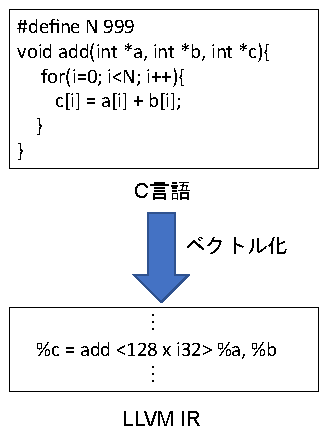
\includegraphics[scale=0.7]{image/Auto_vectorize.pdf}
    \caption{LLVMによる自動ベクトル化例}
    \label{fig:LLVM_auto_vec}
\end{figure}

%また,LLVM IRにおけるベクトル処理の流れを図%フローチャートを作って載せる
%に示す.
また,LLVM IRでは対象配列の全要素に演算を行うための制御を行っている.例えば対象配列要素数が400とし,一度にベクトル演算を行う個数を128とする.この場合,128個を対象としたベクトル演算を3回行う.その結果ベクトル演算によって384個の要素を演算するが,16個の要素が残ることになる.この余りに関しては逐次処理を16回繰り返す処理を行う.これによってすべての配列要素の演算を可能にしている.

LLVMではベクトル化されたLLVM IRからベクトル命令を生成することが可能である.ベクトル化されたLLVM IRからRISC-VのV拡張命令のベクトル命令の生成にも対応しており,C言語等で記述した配列加算プログラム等を自動でRISC-Vのベクトル化アセンブリコードに変換することが可能である.本研究ではこの機能を再利用することによってベクトル拡張付きRISC-Vのベクトル命令を出力する.